\section{Lezione 24 - 16/11/2023} 
\subsection{Grafo (Fortemente) Connesso}
Dato un Grafo $G = (V,E)$ esso è detto fortemente connesso $\iff$ 
$$ \forall (u,v) \in V, (u,v) \text{ sono reciprocamente raggiungibili}$$
(Useremo il termine \textbf{fortemente} solo per quanto riguardo i grafi \textbf{orientati})
%Un caso molto favorevole alle componenti fortemente connesse sono i grafi non orientati, quindi quei grafi che hanno archi sia entranti che uscenti con un simbolo solo, poiche $u \Rightarrow v$ e $u \Leftarrow v$.

%In questo caso dunque la \textbf{reciproca raggiungibilita}(RR) coincide con la \textbf{raggiungibilita}(R) nei grafi non orientati. $RR = R$.

Nel caso di grafi \textbf{non orientati} la \textbf{reciproca raggiungibilita}(RR) coincide con la "normale" \textbf{raggiungibilita}(R), (RR=R), dato che se $u \sim v \Rightarrow v \sim u $.

\begin{figure}[H]
    \centering
    \begin{subfigure}[b]{0.35\textwidth}
        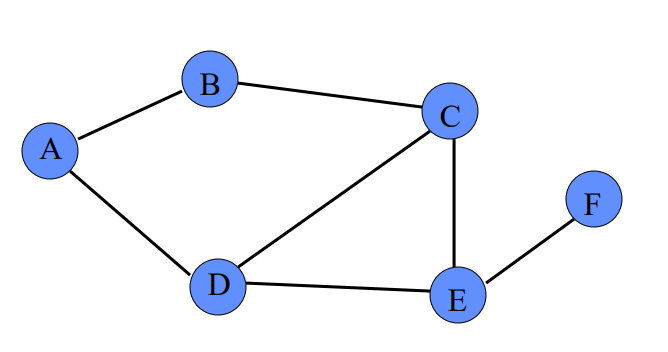
\includegraphics[width=\textwidth]{GrafoConnesso} 
        \caption{Grafo Connesso}
    \end{subfigure}
    \hfill
    \begin{subfigure}[b]{0.35\textwidth}
        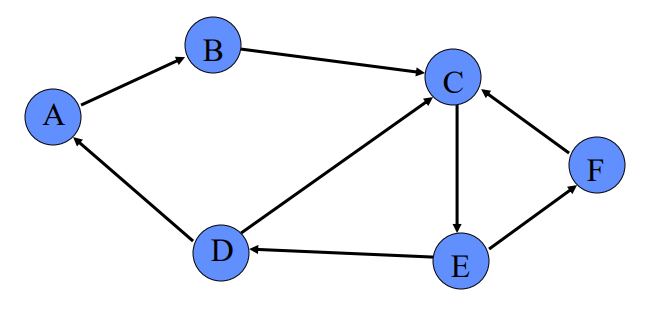
\includegraphics[width=\textwidth]{GrafoFortementeConnesso} 
        \caption{Grafo Fortemente Connesso}
    \end{subfigure}
\end{figure}

\subsubsection{Sottografi (Fortemente) Connessi}
In un Grafo non (fortemente) connesso, può essere presente un \textbf{sottografo} (fortemente) connesso, nella figura seguente possiamo notare un grafo non connesso ma che presenta due sottografi connessi.
\begin{figure}[H]
    \centering
    \begin{subfigure}[b]{0.20\textwidth}
        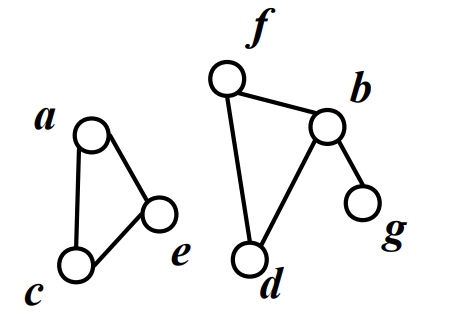
\includegraphics[width=\textwidth]{GrafoConnessoPrimo} 
		%\caption{Grafo non Connesso}
    \end{subfigure}
\end{figure}

%TODO: Da capire che cazzo sta scritto
%
%
%
%
%\subsection{Componenti Fortemente Connesse tra grafi orientati e non orientati}
%Per un grafo orientato, 2 vertici sono mutualmente raggiungibili solamente se esiste un ciclo.
%Ogni coppia di vertici nella mutua raggiungibilita e compresa nell'insieme della raggiungibilita tra vertici
 %$$RR \subseteq R$$ ma non $$RR not \supseteq R$$.
%
%
%
%
%



%\newtheorem{proprieta}{Proprieta}
%\begin{proprieta}
%	Anche in grafi che non hanno una forte connessione (insieme di archi al suo interno), possono esistere sottografi fortemente connessi.
%\end{proprieta}



\subsection{Componente (Fortemente) Connessa}

Dato un grafo $G=(V,E)$ e un suo sottografo $G^{\prime}$, $G^{\prime}$  è C(F)C di $G$ $\iff$ 
\begin{itemize}
	\item È un sottografo (fortemente) connesso
	\item È Massimale
\end{itemize}


%\newtheorem{compfortconn}{Definizione}
%\begin{compfortconn}
%	Dato un grafo $G$, $\exists G^{\prime}$ CFC di $G \iff$ 
%		-Esso e fortemente connesso
%		-Esso e massimale
%\end{compfortconn}

\paragraph{Cosa significa Massimale?}
$G^{\prime}$ è un sottografo \textbf{massimale} se non esiste un altro sottografo fortemente connesso di $G$ che contiene $G^{\prime}$ come sottografo.\bigskip

In poche parole vuol dire che non esiste un altro sottografo C(F)C con gli stessi vertici e stessi archi; nel caso in cui si aggiungesse un vertice si verrebbe a perdere la proprietà di massimale.

\begin{figure}[H]
    \centering
    \begin{subfigure}[b]{0.35\textwidth}
        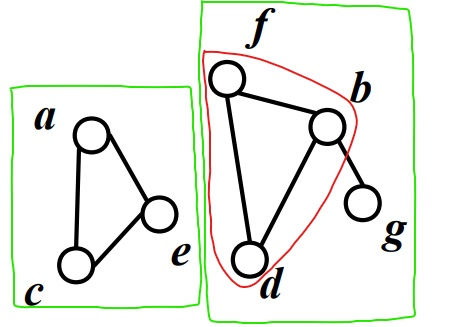
\includegraphics[width=\textwidth]{CFCEsempio} 
		%\caption{Grafo non Connesso}
    \end{subfigure}
\end{figure}
Consideriamo il seguente grafo, come già osservato non è connesso ma sono presenti dei sottografi connessi, andiamo a verificare quale di questi siano C(F)C.\smallskip

\begin{itemize}
	\item (a,c,e): è \textbf{componente connessa} poiché è un sottografo connesso, inoltre è \textbf{massimale} poiché non possiamo aggiungere altri vertici/archi.\smallskip
	
	\item (b,d,f,g): è componente connessa per gli stessi motivi di sopra \smallskip
	
	\item (b,d,f): \textbf{non è componente connessa}, è un sottografo 
	connesso ma non è massimale, poiché il sottografo (b,d,f,g) contiene a sua volta questo sottografo.
\end{itemize}

\paragraph{Caso Orientato} Nel caso dello stesso Grafo ma orientato avremo i seguenti CFC:
\begin{figure}[H]
    \centering
    \begin{subfigure}[b]{0.35\textwidth}
        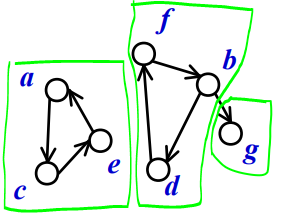
\includegraphics[width=\textwidth]{CFCOrientato} 
		%\caption{Grafo non Connesso}
    \end{subfigure}
\end{figure}
Rispetto al caso precedente il grafo (b,d,f,g) non è più cfc poiché se aggiungessimo il nodo $g$ non sarebbe più sottografo connesso ma solo massimale, inoltre il sottografo in cui è presente solo $g$ è cfc poiché non è compreso in nessun altro grafo.

\subsection{Raggiungibilità nei C(F)C}

Dato $u$ e $v$ in un grafo $G$, $u$ e raggiungibile da $v$ in $G \iff$ 
\smallskip

\begin{center}
	Esiste un percorso ($\pi$) da un qualsiasi vertice \\della CFC(u) ad un qualsiasi vertice della CFC(v).
\end{center}\bigskip

In altre parole, stiamo collegando solo i vertici che appartengono a entrambe le Componenti Fortemente Connesse (CFC), senza alcun altro collegamento tra di esse. Quindi, se prendiamo due vertici arbitrari ($z$  dalla CFC di $u$ e $k$ dalla CFC di $v$), il percorso che stiamo considerando li connetterà le CFC.\smallskip

Il vantaggio è di poter rappresentare il grafo (magari con molti vertici), in maniera piu compatta e leggera.\bigskip

Dunque il grafo "compatto" sarà espresso così:

$$G_{CFC} = (V_{CFC}, E_{CFC})$$.

Le sue componenti saranno:\medskip

\begin{itemize}
    \item $V_{VFC}$: contiene un nodo per ogni CFC di $G$
    \item $E_{CFC}$: $(u,v)| u,v \in V_{CFC}, \exists $ un arco in $E$ da un vertice in $u$ a un vertice in $v$.
\end{itemize}\bigskip

Prendiamo il grafo precedente e proviamo a costruire il grafo CFC:

\begin{figure}[H]
    \centering
    \begin{subfigure}[b]{0.75\textwidth}
        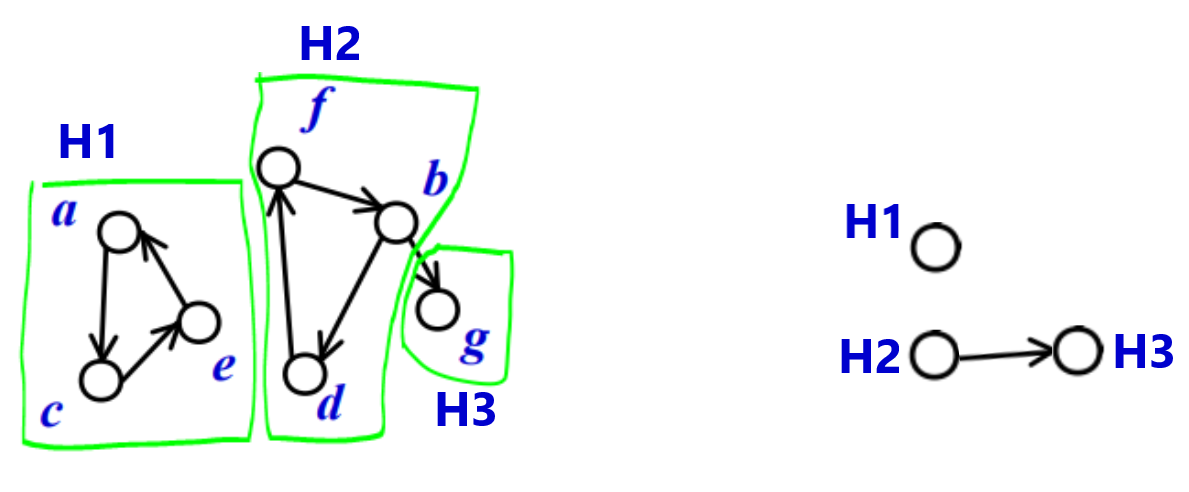
\includegraphics[width=\textwidth]{GrafoCFC} 
		%\caption{Grafo CFC}
    \end{subfigure}
\end{figure}\smallskip

Possiamo notare come per ogni CFC è stato preso un vertice che lo rappresenta, e l'unico arco serve a "simulare" la connessione tra il nodo $b$ e il nodo $g$ che appartengono a due CFC diverse.

\paragraph{Proprietà} \underline{Il grafo delle CFC di $G$ è un grafo \textbf{aciclico}}.

%\newtheorem{corollcfc}{Proprieta}
%\begin{corollcfc}
%	La proprieta di questo GrafoCFC e che nella rappresentazione non esisteranno cicli.
%\end{corollcfc} 


\subsubsection{Parrallelismo con Algebra}
Se fossimo in Algebra, i sottografi CFC sarebbero delle sottoclassi dell'insieme quoziente che è il grafo G stesso. In poche parole i $V_{CFC}$ vanno a rappresentare una classe di equivalenza nella quale tutti i vertici sono in relazione con la classe attraverso la reciproca raggiungibilita (RR).
La RR dunque sarà una relazione di equivalenza.

%FINE CORREZIONE PARTE DI ALEX 
\subsection{Costruire un Grafo CFC}
Dato un grafo $G=(V,E)$ vogliamo calcolare l'insieme delle componenti fortemente connesse, ognuno degli elementi appartente all'insieme è \textbf{un sottografo \underline{indotto}}, poiché se prendiamo come esempio $CFC(U)$ sarà composto da:\smallskip

\begin{itemize}
    \item $V_u$=$\{v \in V| \text{ v è reciprocamente raggiungibile con } u\}$
    
    \item $E_u$=$E \cap (V_u x V_u)$ [è proprio la definizione di grafo indotto]
\end{itemize}\medskip

Come possiamo notare la difficoltà sta nel calcolare $V_u$ poiché $E_u$ è facilmente ricavabile dalla definizione.

%Per la costruzione del grafo avremo bisogno delle componenti fortemente connesse ($V_{CFC}$) e degli archi che le connettono. La parte piu difficile e quella di trovare le componenti fortemente connesse.
%Per lo scorrimento degli archi devo verificare se $\forall(u,v)$, $u$ ha arco in $v$ e $v$ ha arco in $u$.

Inoltre c'è la complessità di calcolo è diversa a secondo del grafo, per un grafo orientato, due vertici sono mutualmente raggiungibili solamente se esiste un ciclo.
Ogni coppia di vertici nella mutua raggiungibilita è compresa nell'insieme della raggiungibilita tra vertici.
 $$RR \subseteq R \text{ ma non } RR \not \supseteq R$$.

\subsection{Costruzione Grafo CFC - Caso non Orientato}
Per un grafo non orientato e piu semplice trovare questo grafo poiche avremo la proprieta sopra menzionata che $RR = R$, quindi qualsiasi arco sara automaticamente reciproco.

\newtheorem{ragnonorientato}{Ragionamento}

\begin{ragnonorientato}
	Possiamo eseguire dunque la DFS sul grafo non orientato per trovare la raggiungibilita, che ricordiamo equivalere alla raggiungibilita reciproca.
\end{ragnonorientato}

La DFS creera un insieme di alberi che andranno a stabilire il numero di CFC.
Ogni albero ha dunque l'insieme dei vertici fortemente connessi ($V_{CFC}$). E ognuno di essi costituira un array(CC) che associa un numero naturale ad ogni sottoalbero creato dalla DFS.

$$CC : V_{CFC} \rightarrow N$$


\begin{lstlisting}[language=Java]
	DFS_Visit(S,i)
		CC[s]=i
		DFS_Visit(...,i)
\end{lstlisting}

Con questa modifica del codice possiamo cosi costruire $V_{u}$, dove $V_u = {v \in V | CC[v] = CC[u]}$


Questo algoritmo impieghera tempo lineare su G e tempo di costruzione dell'array sempre lineare, sommato alla visita.

L'array $k$ non sara vuoto, ma avra come elemento minimo di creazione 1 e elemento massimo $|V|$.

\newtheorem{consCFCnonorientato}{Suggerimento}

\begin{consCFCnonorientato}
	Nella DFS normale si partira con i = 1 e incrementera ogni volta che incontra una sorgente bianca.
\end{consCFCnonorientato}

\subsection{Ragionamento per un grafo Orientato}
Questo stesso ragionamento non puo valere per un grafo orientato poiche da subito non e vero che ogni albero Della DFS e CFC di G.
Dobbiamo ragionare quindi su diverse proprieta che abbiamo a disposizione:
\newtheorem{ideaorientato}{Idea}
\begin{ideaorientato}
	\item Al termine di una DFS su G siamo sicuri che 
		\subitem Se $u$ e $v \in$ alla stessa componente, allora $u$ e $v \in$  allo stesso albero
		Questo vuol dire che una stessa componente non puo stare in piu alberi diversi. Il problema che si propone dunque e dividere gli alberi nelle loro CC diverse, nonstante la DFS crei un albero con piu CC insieme.
		Dimostrazione nella prossima lezione
\end{ideaorientato}


